
\documentclass[13pt,compress]{beamer}
% deactivate beamer navigation
%\setbeamertemplate{navigation symbols}{}
%\usepackage{geometry}
%\geometry{papersize={180mm, 135mm}, top=-1.5mm} % 210mm, 297mm

\usepackage[nospeakermargin]{../../style/lmu-lecture}

\setbeamertemplate{frametitle}{\expandafter\uppercase\expandafter\insertframetitle}
%\useoutertheme{metropolis}
% remove section slides
\AtBeginSection[]
{
  \begin{frame}<beamer>
    \frametitle{Supervised Learning III}
    \tableofcontents[currentsection]
  \end{frame}
}
% includepdf slides, pagecommad will set counter for framenumber
\usepackage{pdfpages}
\includepdfset{trim=0mm 0mm 0mm 0mm, pagecommand={\global\setcounter{framenumber}{\value{page}}}}
% trim=0mm 6mm 0mm 0mm, offset=0 15,
% add footer:
\usepackage{framed, color}
\usepackage{xcolor}
%\iffalse
\usepackage{transparent}

\setbeamertemplate{footline}[text line]{%
    \noindent\hspace*{\dimexpr-\oddsidemargin-1in\relax}%
     \colorbox{white}{
     \makebox[\dimexpr\paperwidth-2\fboxsep\relax]{
     \color{black}
     \begin{minipage}[c][2.5ex][b]{0.5\linewidth}
       \secname
     \end{minipage}
     \hfill\begin{minipage}[c][2.5ex][b]{0.5\linewidth}
       \flushright
       \insertframenumber{}~/~\inserttotalframenumber~~
     \end{minipage}
     }}%
  \hspace*{-\paperwidth}
  }

%\fi

\title{Supervised Learning III}
\author{Essential Data Science Training}
%\institute{Essential Data Science Training}
\date{}



\begin{document}
\setbeamercolor{background canvas}{bg=}

% General remark: hyperlinks in included pdfs are not clickable anymore in the combined pdf

\frame{\titlepage}

\section{Introduction to Interpretability}
\includepdf[pages={2-6}, trim=0mm 0mm 45mm 0mm]{../../material/lecture_iml/slides-pdf/slides01-intro-motivation.pdf}
\includepdf[pages={2-15}, trim=0mm 0mm 45mm 0mm]{../../material/lecture_iml/slides-pdf/slides03-intro-dimensions.pdf}
\section{Bascis: Dependence vs. Interactions}
\includepdf[pages={3, 9-16, 19-20}, trim=0mm 0mm 45mm 0mm]{../../material/lecture_iml/slides-pdf/slides04-intro-correlation.pdf}
\includepdf[pages={2-9}, trim=0mm 0mm 45mm 0mm]{../../material/lecture_iml/slides-pdf/slides05-intro-interaction.pdf}
\section{Feature Effects - ICE and PDP}
\includepdf[pages={2-6}, trim=0mm 0mm 45mm 0mm]{../../material/lecture_iml/slides-pdf/slides01-fe-intro.pdf}
\includepdf[pages={2-last}, trim=0mm 0mm 45mm 0mm]{../../material/lecture_iml/slides-pdf/slides03-fe-pdp.pdf}
\includepdf[pages={2-4}, trim=0mm 0mm 45mm 0mm]{../../material/lecture_iml/slides-pdf/slides04-fe-pdp-comments.pdf}
\section{Loss-based Feature Importance - PFI}
\includepdf[pages={3}, trim=0mm 0mm 45mm 0mm]{../../material/lecture_iml/slides-pdf/slides01-fi-intro.pdf}
\includepdf[pages={2-10}, trim=0mm 0mm 45mm 0mm]{../../material/lecture_iml/slides-pdf/slides02-fi-pfi.pdf}
\section{Local Explanations - LIME}
\includepdf[pages={4, 16-20, 7-8, 10, 12-14}, trim=0mm 0mm 45mm 0mm]{../../material/lecture_iml/slides-pdf/slides04-le-lime.pdf}
\includepdf[pages={2-4}]{../../material/lecture_iml/slides-pdf/slides05-le-lime-example.pdf}
\section{Feature Filtering and Feature Selection}
\includepdf[pages={4}, trim=0mm 0mm 45mm 0mm]{../../material/lecture_sl/slides-pdf/slides-fs-introduction.pdf}
\includepdf[pages={2, 4, 9}, trim=0mm 0mm 45mm 0mm]{../../material/lecture_sl/slides-pdf/slides-fs-filters1.pdf}
\includepdf[pages={5-6}, trim=0mm 0mm 45mm 0mm]{../../material/lecture_sl/slides-pdf/slides-fs-filters2.pdf}
\includepdf[pages={6-7}, trim=0mm 0mm 45mm 0mm]{../../material/lecture_sl/slides-pdf/slides-fs-introduction.pdf}
\includepdf[pages={4-9, 13}, trim=0mm 0mm 45mm 0mm]{../../material/lecture_sl/slides-pdf/slides-fs-wrapper.pdf}



\end{document}
